\section{Conclusion}
In conclusion, the current application is a web application that gives teachers the ability to create sessions which contain questions that are relevant to a lecture. The application implements all the features from the primary goals for the project. The application supports the use of WebSockets and can have multiple students participate in a session. The sessions have a layout that supports both mobile devices and computers. While the admin portion of the application is designed for pc users, it works on mobile. The application has a drawing tool, that is designed to be used both to answer questions and create questions about certain algorithms and data structures in the courses DAT110 and DAT200. The application stores the result of questions and sessions. This data can be used by the teacher to check if students understand the material in the course. Other features such as supporting OpenID Connect for student authorization, student feedback, and localization support were added during the development because these features worked well with the planned structure of the application. 
\\[11pt]
During the development of the application, a lot of different tools had to be used. In general, the group had very little to no experience working with the tools used in the project. This includes developing single page web applications using Vue, using Socket.IO for the WebSocket functionality of the sessions, and OAuth in order to authenticate students using their Feide users. By the end of the project, the group members have gained experience working with these tools, and the group has, in general, learned a lot more about modern web tools and frameworks. The group has learned a lot about how to structure larger software projects, and working in teams.
\\[11pt]
One of the challenges with implementing solution checking and generating is that user input can create objects which do not fit with the actual data structure. For instance, when answering a question about binary trees, they can create nodes which have more than two children; they can create trees with several roots, or create cycles in the tree. This made it a lot harder to create correct algorithms because there were many edge cases for each question type. 

\subsection{Future Development}

\subsection{Server side}
\subsubsection{Server}
Due to limited time and resources a decision was made to make a single server and make it responsible for handeling all traffic from the users. This will not be a problem for the server load for the use case at the moment. If the web app should be scaled up to include subjects for the entire university and all its student, or scaled up even further. The server should be split up into microservices, where each service is its own server serving a single purpose. For example everything that has to do with login is its own server and everything that has to do with running an active session is on its own server. These microservices could be placed inside their own docker container and with the use of kuberenetes the servers would scale up and down depending on the amount of traffic. Since the amount of work required in R\&D for all the other features and techologies we used, this was something we would want to do, but simply just didn't have enough time to get done.
\\[11pt]
Another factor that would limit the scalability for the server is the use of a map for connected users and the map for active sessions. After some testing this will not be a problem where the use case is a couple of classes and a couple of active session at the same time. If the traffic where to be scaled up for the entire university or for multiple universities, there could be a problem since the limiting factor would be the available ram on for the server. A way to avoid this would be to redesign how sessions and users are stored in the database, allowing that information that is stored in ram now to be stored directly in the database. 
\subsubsection{Database}
Another feature that would suffer if the web app scaled up is the database. The database is using SQLite3 where the limit is 50000 requests per second\cite{SQLite:faqQ19}. This could be a limit if the traffic is scaled up enough, and there should be looked into using another type of database that uses a server to handle the requests. This would also allow the database to be split up into smaller databases and not a single schema for the entire application. Currently the ids are in incremental integers. In the future it would be beneficial to change these to GUID or UUID.\cite{UUIDE}

\subsection{Client}

\subsubsection{Anonymous Login}
\begin{figure}[H]
    \centering
    \begin{subfigure}{0.60\linewidth}
        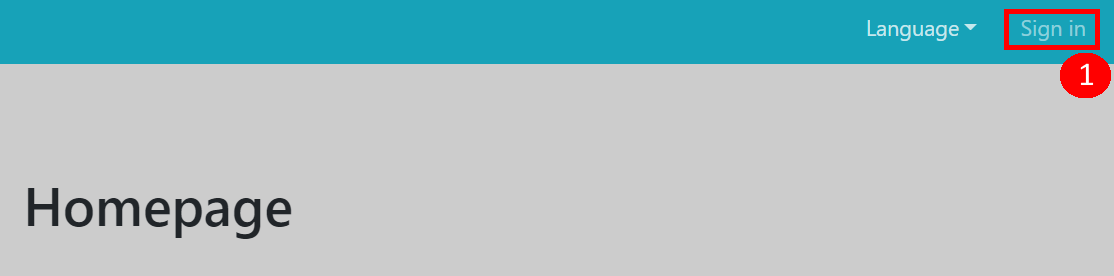
\includegraphics[width=\linewidth]{/userManual/client/login/mainpage}
       	\caption{}
		\label{fig:annoMainPage}	
    \end{subfigure}
    \begin{subfigure}{0.60\linewidth}
        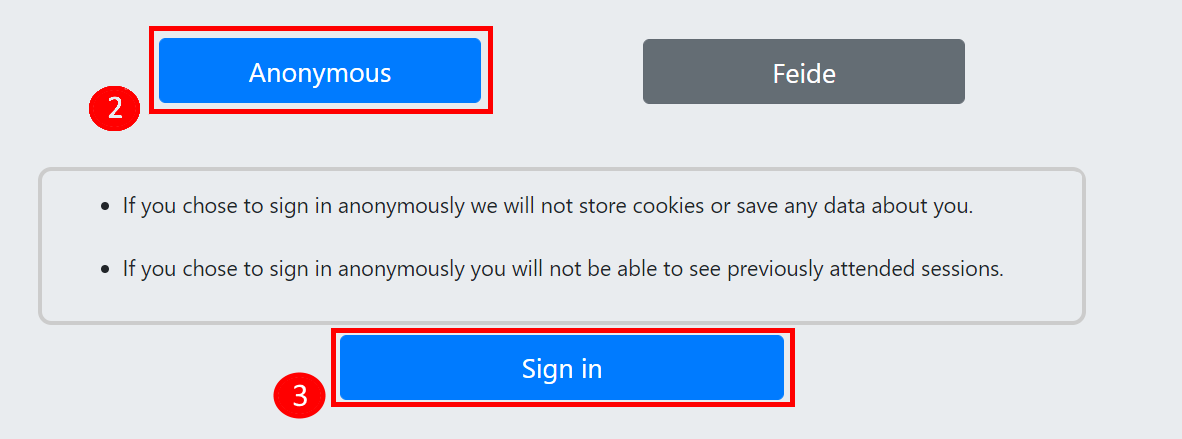
\includegraphics[width=\linewidth]{/userManual/client/login/annoLogin}
      	\caption{}
		\label{fig:annoLogin}	
    \end{subfigure}
    \begin{subfigure}{0.60\linewidth}
    	
\includegraphics[width=\linewidth]{/userManual/client/login/annoResult}
    	\caption{}
    	\label{fig:annoResult}	
    \end{subfigure}
\end{figure}

\begin{userManualItemlist}
	\item[Step I.] Click the Sign in button (1). (Figure: \ref{fig:annoMainPage})
	\item[Step II.] Click the button (2) labeled “Anonymous”. (Figure: \ref{fig:annoLogin})
	\item[Step III.] Click the button (3) labeled “Sign in” to anonymously log in to the page. (Figure: \ref{fig:annoLogin})
	\item[Step IV.] If the login was successful, the navigation bar displays a random animal name. (Figure: \ref{fig:annoResult})
\end{userManualItemlist}

\subsubsection{Feide Login}
\begin{figure}[H]
    \centering
    \begin{subfigure}{0.60\linewidth}
        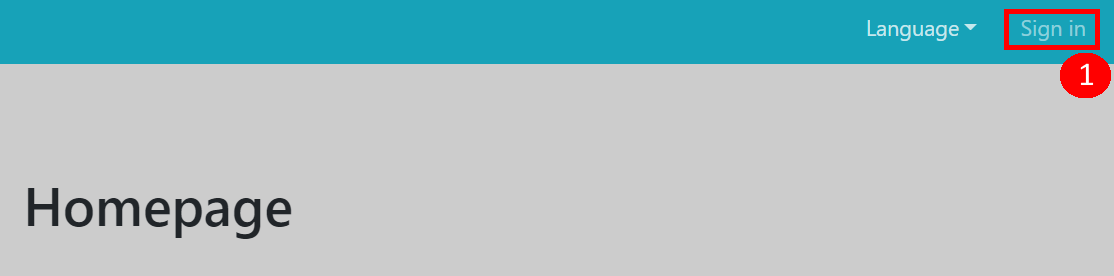
\includegraphics[width=\linewidth]{/userManual/client/login/mainpage}
       	\caption{}
		\label{fig:feideMainPage}	
    \end{subfigure}
    \begin{subfigure}{0.60\linewidth}
        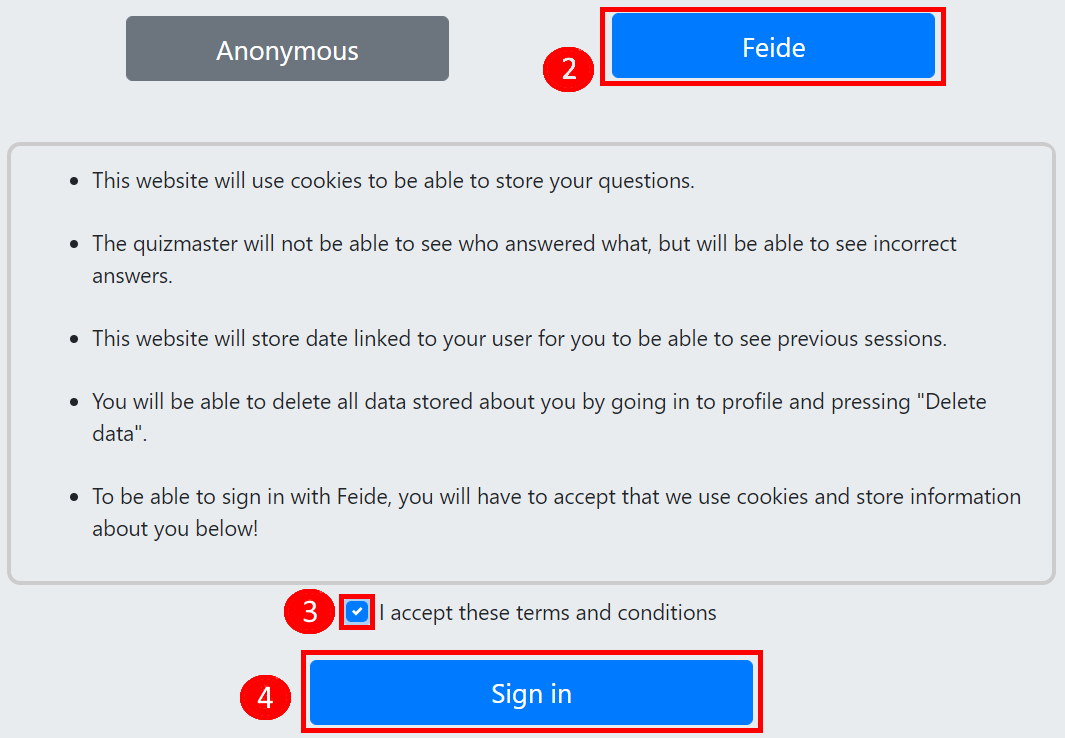
\includegraphics[width=\linewidth]{/userManual/client/login/feideLogin}
      	\caption{}
		\label{fig:feideLogin}	
    \end{subfigure}
     \begin{subfigure}{0.60\linewidth}
        
\includegraphics[width=\linewidth]{/userManual/client/login/feideResult}
      	\caption{}
		\label{fig:feideResult}	
    \end{subfigure}
\end{figure}

\begin{userManualItemlist}
	\item[Step I.] Click the Sign in button (1). (Figure: \ref{fig:feideMainPage})
	\item[Step II.] Click the button (2) labeled “Feide”. (Figure: \ref{fig:feideLogin})
	\item[Step III.] Read through the terms of use!  
	\item[Step IV.] Click the radio button (3). (Figure: \ref{fig:feideLogin})
	\item[Step V.] Click the button (4) labeled “Sign in”. (Figure: \ref{fig:feideLogin}) 
	\item[Step VI.] Follow the instructions given and log in to your Feide account.
	\item[Step VII.] If the login was successful, the navigation bar displays your Feide name. (Figure: \ref{fig:feideResult})
\end{userManualItemlist}


\subsubsection{Joining a Session}


\subsubsection{User Profile}
\begin{figure}[H]
	\begin{subfigure}{0.80\linewidth}
		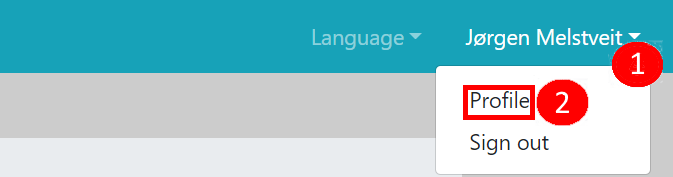
\includegraphics[width=\linewidth]{userManual/client/userProfile/accessUserProfile}
		\caption{}
		\label{fig:accessUserProfile}	
	\end{subfigure}
	\begin{subfigure}{0.80\linewidth}
		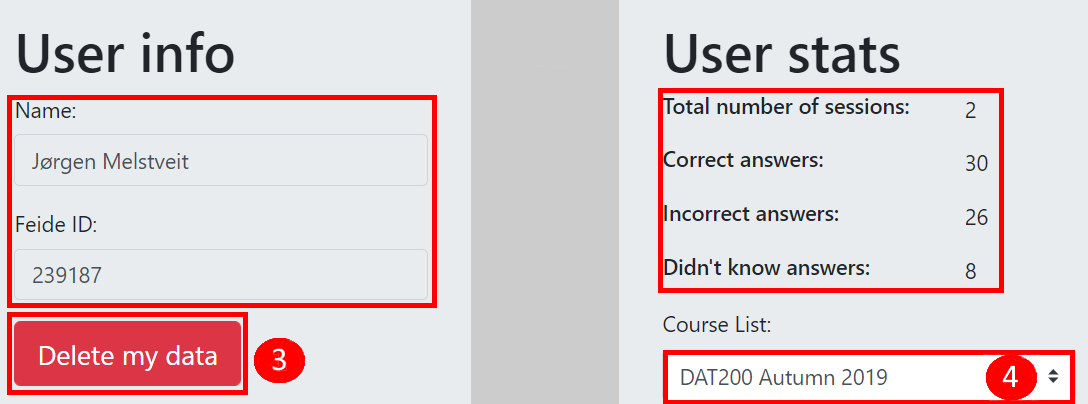
\includegraphics[width=\linewidth]{userManual/client/userProfile/profile}
		\caption{}
		\label{fig:profilePage}
	\end{subfigure}
\end{figure}

\begin{userManualItemlist}
	\item[Step I.] You need to be signed in to your Feide Account to access your user account. 
	\item[Step II.] Click the button (1) with your Feide name on the navigation bar. (Figure: \ref{fig:accessUserProfile})
	\item[Step III.] Click "Profile" button (2). (Figure: \ref{fig:accessUserProfile})
	\item[Step IV.] View user info. The user info contains the Feide username and Feide name. (Figure: \ref{fig:profilePage})
	\item[Step V.] Click the button (3) labeled "Delete my data" if you want to delete your user data on the application. This includes your old session data. (Figure: \ref{fig:profilePage})
	\item[Step VI.] View user stats. The stats includes your total number of sessions, the total amount of questions you answered correctly, the total amount of questions you answered incorrectly and how many times you answered "I don't know". (Figure: \ref{fig:profilePage})
	\item[Step VII.] Choose the course you want to view session data for (4). If you participated in a session corresponding to the selected course, a list of sessions will appear. (Figure: \ref{fig:profilePage})
	\item[Step VIII.] Click on the selected session you want to view your answers for.
\end{userManualItemlist}

\subsubsection{Sandbox}
\begin{figure}[H]
	\begin{subfigure}{0.70\linewidth}
		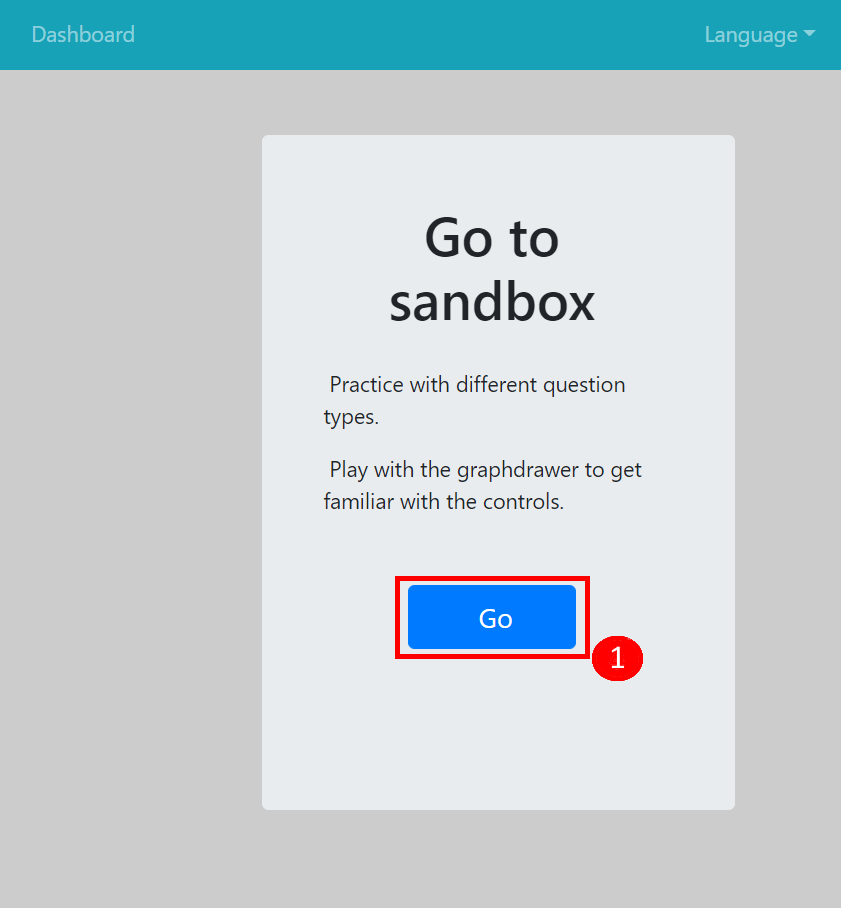
\includegraphics[width=\linewidth]{userManual/client/sandbox/goToSandbox}
		\caption{}
		\label{fig:goToSanbox}
	\end{subfigure}
	\begin{subfigure}{0.80\linewidth}
		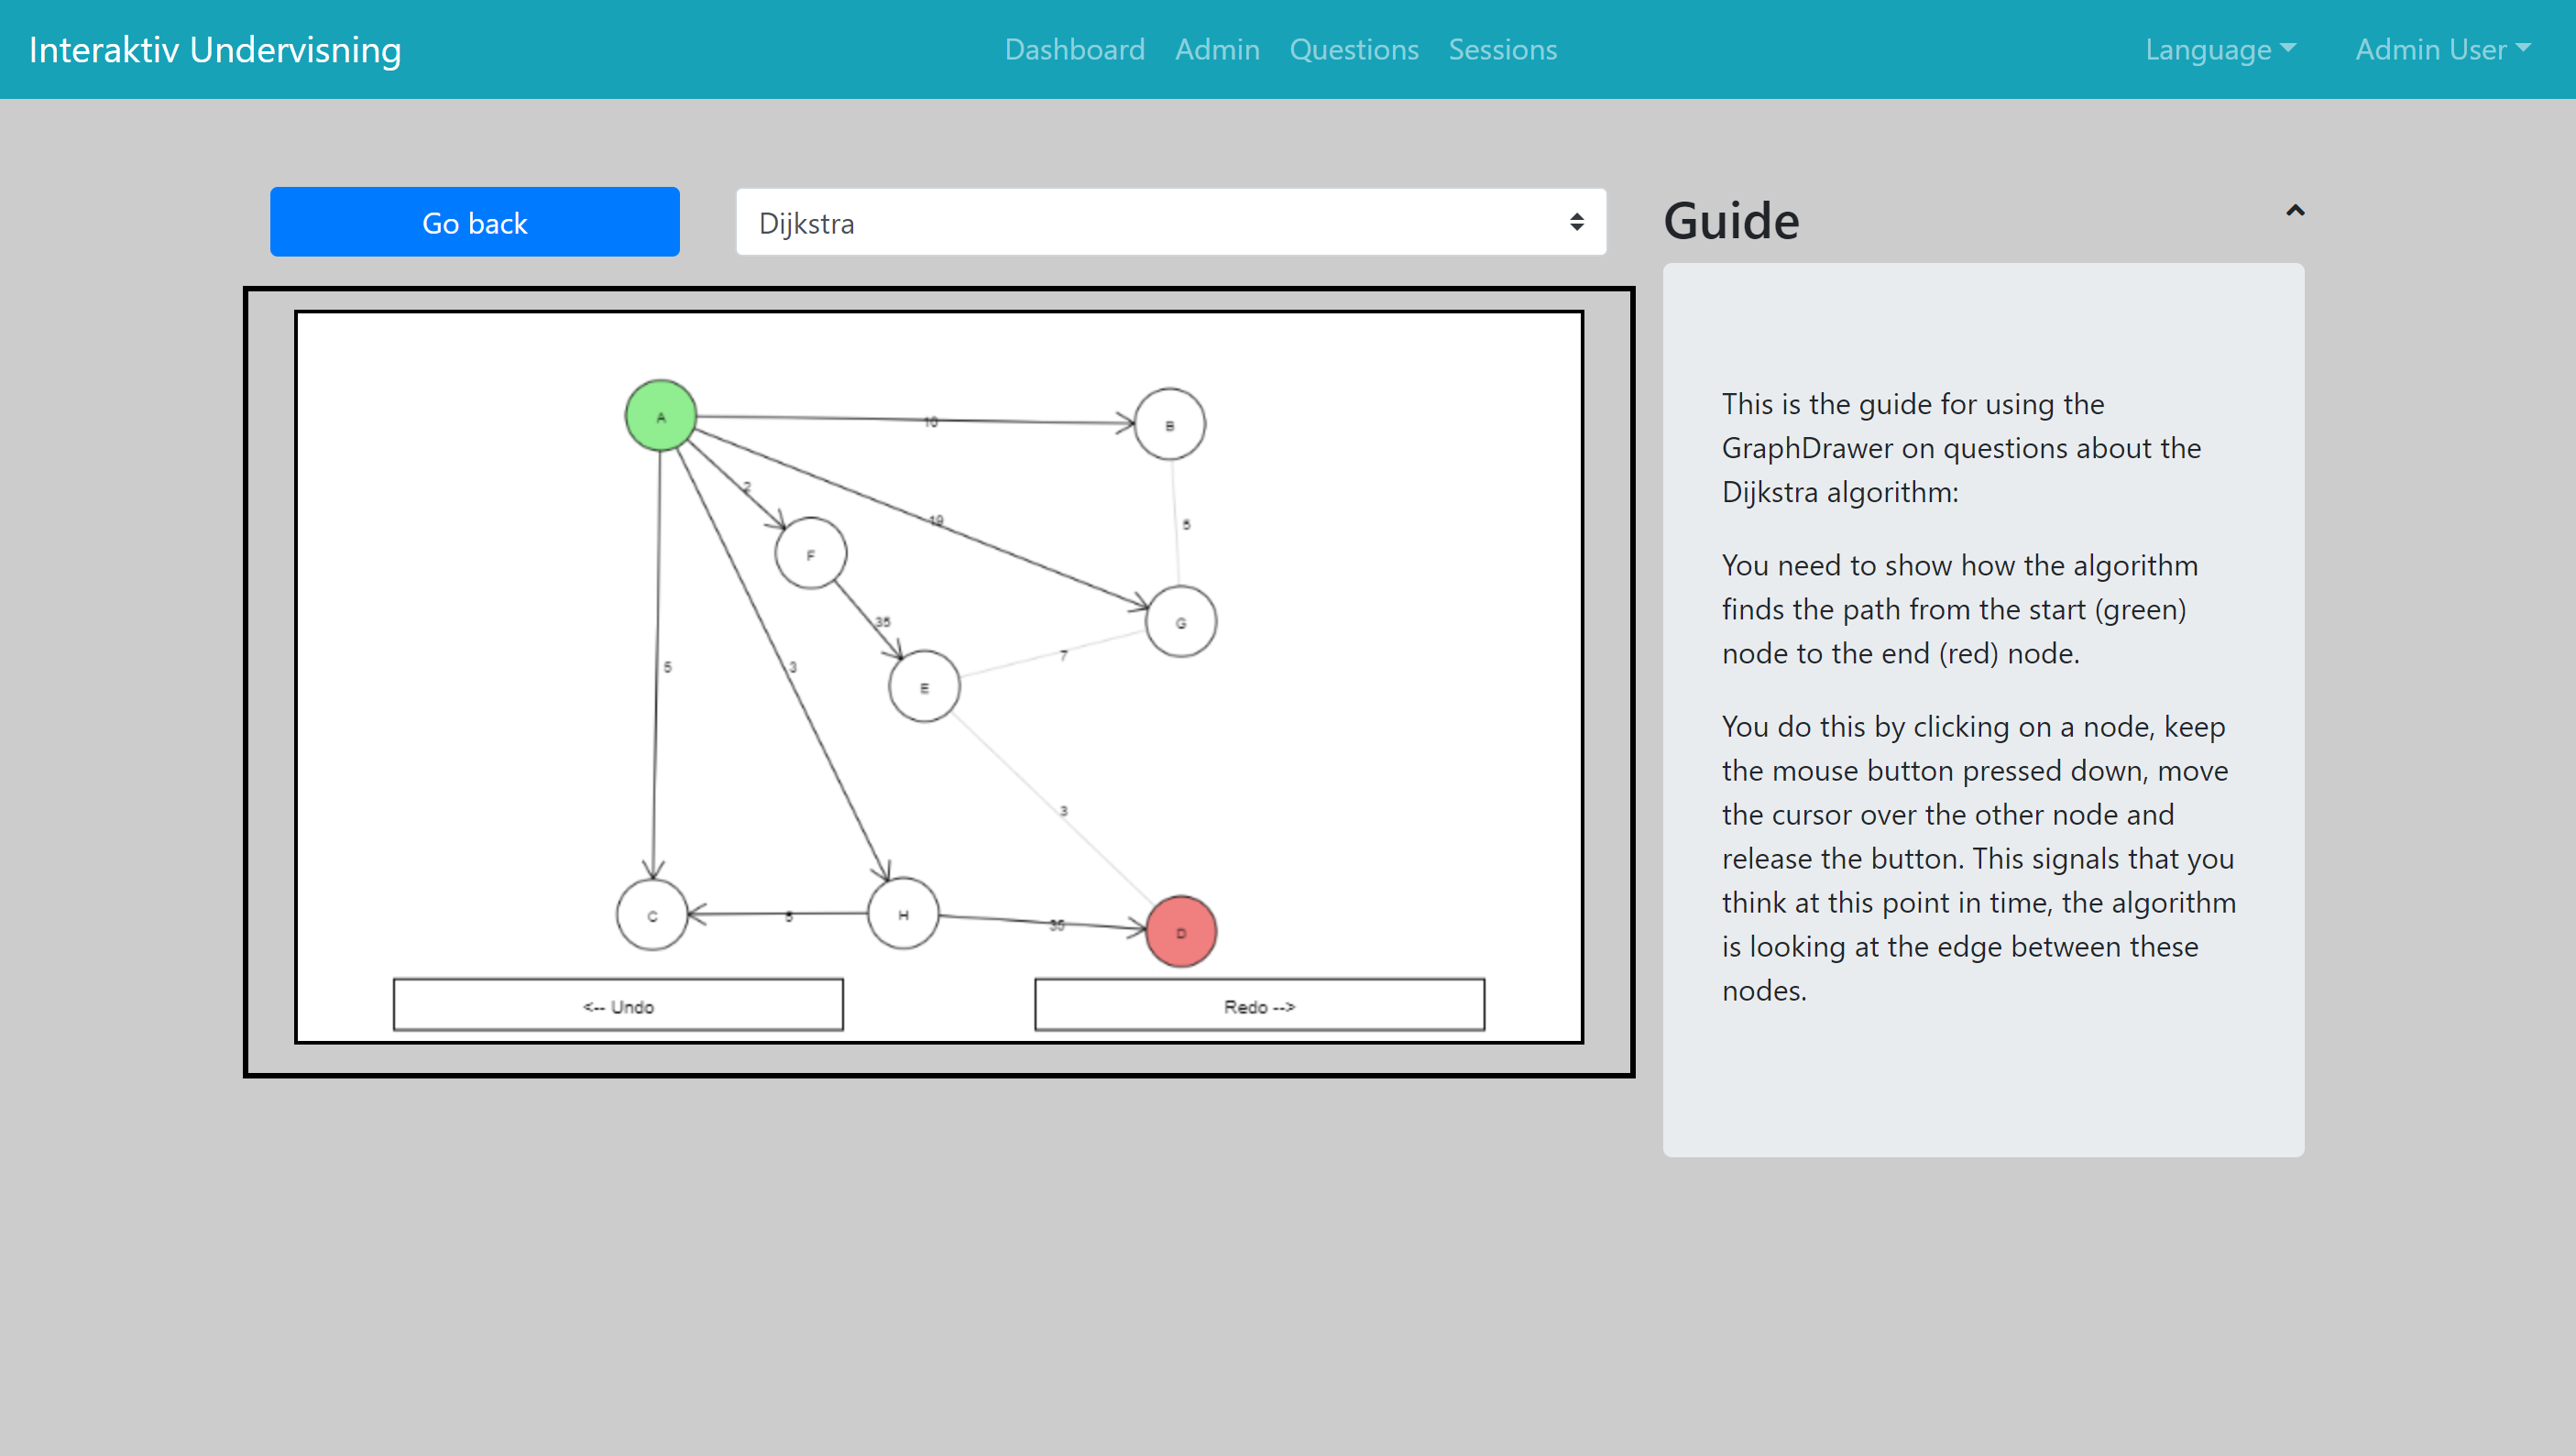
\includegraphics[width=\linewidth]{userManual/client/sandbox/sandbox}
		\caption{}		
		\label{fig:sandbox}
	\end{subfigure}
\end{figure}

\begin{userManualItemlist}
	\item[Step I.] Navigate to the dashboard page.
	\item[Step II.] Click the button (1) labeled "Go" within the "Go to sandbox" area. (Figure: \ref{fig:goToSanbox})
	\item[Step III.] Select the question type you want to practice. (2) (Figure: \ref{fig:sandbox})
	\item[Step IV.] Read the user guide for the chosen question type. (3) (Figure: \ref{fig:sandbox})
	\item[Step IV.(2)] Some question type have access to a settings together with the user guide. If this is the case then you have the option of changing the question types initial settings. (Figure: \ref{fig:sandbox})
	\item[Step V.] Practice solving exercises with the given tools. (4) (Figure: \ref{fig:sandbox})
	\item[Step VI.] When you are finished exit the sandbox by clicking the button (5) labeled "Go back". (Figure: \ref{fig:sandbox})
\end{userManualItemlist}


\subsection{Testing}
\subsubsection{Unit-tests}
At current state, the application does not have nearly as many unit-tests as it should. Due to limited time and resources writing unit tests became more of an afterthought in comparison to getting the server functionality working. The unit tests that the project currently has are unit tests for the different algorithms and data structures, and these tests have been primarily used in order check that these work the way they should. Areas in the application where there should be unit tests, but currently does not have any are in the Validation Checker and the Solution Checker residing on the server. In the future it might be beneficial if some tests were made for each question type for both checkers. This would in turn help during debugging if any changes were to affect the checkers when implementing a new type of question.
\subsubsection{End-To-End tests}
It is recommended by Vue to set data-attributes on the html elements that were going to be tested. This is to make it easier for Cypress to select and obtain the correct html element. This is normally a problem since the html elements tend to constantly change their attributes during development in a Vue application. Unfortunately, these data-attributes could potentially present a security risk if they were present in the production build. However, a method of removing these in only the production mode, while keeping them in testing mode was never discovered. This is something to keep in mind for the future development of the application. All the data-attributes used for the current tests have been well documented in a txt file and can be found in the same directory with the rest of the end-to-end tests.\cite{Cypress:BestPractise}\\[11pt] 
The future developers should also be aware that Cypress is intended to be used during development following closely the principles of test-driven development. This means that the test themselves need to be altered a lot to handle the changes done to the html object on the site. Writing E2E-test in Cypress are therefore recommended be begun early in development and not in the middle or at the end of the project.



\subsection{Localization}
When creating the locale files we used a design based on each vue component having their own locale object. This has been a design that worked great, but during development a design flaw was noticed. Some vue components use the same text. This can be seen on buttons, error messages, etc. This could be solved by not just storing locales divided into vue components, but byb also storing comon locale by in it's own object. Even though the file size for each locale file is relatively small, it could reduced more. Another way to expand localization would be to add more locales.

\subsubsection{GraphDrawer}
If new question types are implemented which require the GraphDrawer to keep track of thousands of nodes at the same time, there might be performance issues on some systems. The nodes are currently stored in an array. This means that if the array is searched for a node on the screen, all of the nodes need to be checked, even those on the opposite side of the world. Many operations starting on one node, and ending at a node close to the first node (e.g., selecting nodes by dragging the mouse) would be more performant if a spatial data structure\cite{SpatialDatastructure} was used instead.
\\[11pt]
The current system is designed to work with both touch screens and cursors. Because of this, two choices were made to make the development simpler and less time-consuming.
\begin{enumerate}
    \item When a user needs to enter text or numbers, the JavaScript alert popup is used because this works in all browsers. Some users with a keyboard would have been able to write faster if the GraphDrawer read the input directly. Mobile browsers do not allow a website to open the virtual keyboard from a script. If the mobile browsers change this in the future, a different method for retrieving the user input could be used. Some browsers allow the user to block popups. If this is done, the user can no longer enter text.
    \item For simplicity both desktop and mobile users control the GraphDrawer the same way. User testing can be done to find the gestures which feel the most natural. If the natural way to do something is different depending on the system, different handlers can be implemented.
\end{enumerate}
Every time the world state changes, the canvas is redrawn. Changes outside the camera view should not make the GraphDrawer redraw the world. If only a small part of the world inside the camera view is changed, only that part needs to be redrawn. This has not been implemented because there have not been any performance issues with the current question types.

\subsection{Python}
Python is the programming language used in the DAT100 course at UiS. Students are often struggeling to understand the difference between value type and reference type variables. To make it easier for them to learn, a Python interpreter was implemented which evaluates Python code step by step. Together with the GraphDrawer, the interpreter can be used to ask questions about Python code. The student is able to see whether a variable is value or reference type, and they can see when the value or reference changes. Before implementing a custom interpreter, using the offical Python interpreter was considered. Because of the size of CPython, and the limited time available for this project, it was decided that implementing a custom interpreter was the better option.
\\[11pt]
The following features of Python are supported:
\begin{enumerate}
    \item Variables of the following types: Number, String, Boolean, and Object.
    \item Functions can be defined using the \code{def} keyword. They can either belong to the global scope, or to a class. Functions can return something using the \code{return} keyword.
    \item Classes can be defined using the \code{class} keyword. If a function with the \code{__init__} is defined inside the class, it will be called when a new instance of the class is instantiated.
    \item If statements can be used with the \code{if} keyword. Elif and else statements are also supported.
    \item The following mathematical operators are supported: +, -, /, *.
    \item The following comparison operators are supported: and, or, !, ==, !=, <, >, >=, <=.
    \item Expressions can be grouped and seperated using parenthesis.
    \item Lines starting with a # are treated as comments, and will be skipped by the interpreter.
\end{enumerate}
Significant Python features missing from this interpreter:
\begin{enumerate}
    \item The standard library.
    \item Lists and dictionaries.
    \item Inner classes and functions.
    \item Shared class variables.
    \item Class inheritance.
    \item Loops.
\end{enumerate}
Every operator has the same priority, which means that expressions are always evaluated left to right. This makes some expressions not behave like expected. The following statement results in an error: \code{if 1 + 1 == 2:}, because it is evaluated as \code{1 + (1 == 2)}. To prevent this from happening, parenthesis should be used to order the expressions. The correct statement would be: \code{if (1 + 1) == 2:}.

\subsubsection{Interpreter}
There are three main functions in the interpreter. \code{parseLine} which tries to figure out what the meaning of a code line is. \code{parseLine} is also responsible for deciding which line to parse next. A line can either be a variable assignment which is handled  by the \code{parseLine} function, an expression which is handled by the \code{evaluateExpression} function, or a statement which is handled by the \code{handleKeyword} function. A statement is anything which starts with one of the keywords. An expression is something which can be evaluated to a value.
!! Insert fancy image showing the path code goes trough the interpreter !!
\\[11pt]
An important feature of the interpreter is the scope objects. A scope is an object which stores information about the variables, classes, functions and data inside the scope. Functions are scopes because they can contain private variables. Classes are also scopes, because they can contain functions. Before code can be parsed, a global scope is created. Anything which doesn't belong to a specific scope, is placed in the global scope. Scope data is an array where the index is the address of the stored data, and the value is the stored data. Because the interpreter is implemented in JavaScript, there is no need to seperate value and references types in this array because JavaScript and Python behave the same way. Scope variables are a mapping from variable names to data addresses. Scope functions/classes are mappings from function/class names to function/class objects. Because the interpreter should save the state of the program as steps, the \code{parseLine} function returns an object containing information about the state. If the state was anything other than a function or class definition, the current state is saved as a step.
\\[11pt]
A function is an object with a \code{name}, a list of arguments \code{args}, a list of the code lines belonging to the function \code{code}. A function should also be a scope. The name is used to identify the function. The arguments are used to make sure that when the function is called, the right amount of arguments are passed. The code is stored so the function can be evaluated when it is called. After a function has been defined, the \code{handleKeyword} function returns a state of type \code{"SkipLines"} which tells the caller which lines have already been handled. The interpreter uses the \code{callFunc} function to call Python functions. When a function is called, three things happen in the following order:
\begin{enumerate}
    \item The function arguments are added as local variables. Local variables mean they belong to the function scope. The arguments need to be in the same order as they were defined, because named arguments are not implemented.
    \item Every line found in the functions \code{code} list is parsed using \code{parseLine}. If a \code{return} statement is found before reaching the end, the function will stop parsing, before reaching the end.
    \item The scope of the function is restored to an empty state and data is returned if a return statement was found.
\end{enumerate}
\\[11pt]
A class is an object with a \code{name} and a list of the code lines belonging to the class \code{code}. A class should also be a scope. When a class is defined, the code is also parsed using the \code{parseLine} function. This is done so that any functions within the class is defined in the scope of the class. When the interpreter is instantiating an instance of the class, the \code{instantiateClass} function is called. \code{instantiateClass} will first create a new object which contains all the functions from the class. If the class has a constructor it is called. Finally, the object is returned to the called of \code{instantiateClass}.
!! Write about expression evaluation !!
!! Write about operators !!

\subsubsection{Questions}
!! TODO: Write this :=) !!